%%%%%%%%%%%%%%%%%%%%%%%%%%%%%%%%%%%%%%%%%%%%%%%%%%%%%%%%%%%%%%%%%%%%%%%%%%%%%%%%
%2345678901234567890123456789012345678901234567890123456789012345678901234567890
%        1         2         3         4         5         6         7         8

\documentclass[a4paper, 10pt]{article}
\usepackage[a4paper, margin={2.5cm, 2.5cm}]{geometry}

% The following packages can be found on http:\\www.ctan.org
%\usepackage{epsfig} % for postscript graphics files
%\usepackage{mathptmx} % assumes new font selection scheme installed
%\usepackage{times} % assumes new font selection scheme installed
\usepackage{listings}
\usepackage{graphics}
\usepackage{amsmath}
\usepackage{amssymb}
\usepackage{acro}
\usepackage{enumitem}
\usepackage{graphicx}
\usepackage{wrapfig}
\usepackage{hyperref}
\usepackage{tabularx}
\usepackage{setspace}

\usepackage{color} %use color
\definecolor{mygreen}{rgb}{0,0.6,0}
\definecolor{mygray}{rgb}{0.5,0.5,0.5}
\definecolor{mymauve}{rgb}{0.58,0,0.82}
 
%Customize a bit the look
\lstset{ %
backgroundcolor=\color{white}, % choose the background color; you must add \usepackage{color} or \usepackage{xcolor}
basicstyle=\footnotesize, % the size of the fonts that are used for the code
breakatwhitespace=false, % sets if automatic breaks should only happen at whitespace
breaklines=true, % sets automatic line breaking
captionpos=b, % sets the caption-position to bottom
commentstyle=\color{mygreen}, % comment style
deletekeywords={...}, % if you want to delete keywords from the given language
escapeinside={\%*}{*)}, % if you want to add LaTeX within your code
extendedchars=true, % lets you use non-ASCII characters; for 8-bits encodings only, does not work with UTF-8
frame=single, % adds a frame around the code
keepspaces=true, % keeps spaces in text, useful for keeping indentation of code (possibly needs columns=flexible)
keywordstyle=\color{blue}, % keyword style
% language=Octave, % the language of the code
morekeywords={*,...}, % if you want to add more keywords to the set
numbers=left, % where to put the line-numbers; possible values are (none, left, right)
numbersep=5pt, % how far the line-numbers are from the code
numberstyle=\tiny\color{mygray}, % the style that is used for the line-numbers
rulecolor=\color{black}, % if not set, the frame-color may be changed on line-breaks within not-black text (e.g. comments (green here))
showspaces=false, % show spaces everywhere adding particular underscores; it overrides 'showstringspaces'
showstringspaces=false, % underline spaces within strings only
showtabs=false, % show tabs within strings adding particular underscores
stepnumber=1, % the step between two line-numbers. If it's 1, each line will be numbered
stringstyle=\color{mymauve}, % string literal style
tabsize=2, % sets default tabsize to 2 spaces
title=\lstname % show the filename of files included with \lstinputlisting; also try caption instead of title
}
%END of listing package%
 
\definecolor{darkgray}{rgb}{.4,.4,.4}
\definecolor{purple}{rgb}{0.65, 0.12, 0.82}
 
%define Javascript language
\lstdefinelanguage{JavaScript}{
keywords={typeof, new, true, false, catch, function, return, null, catch, switch, var, if, in, while, do, else, case, break},
keywordstyle=\color{blue}\bfseries,
ndkeywords={class, export, boolean, throw, implements, import, this},
ndkeywordstyle=\color{darkgray}\bfseries,
identifierstyle=\color{black},
sensitive=false,
comment=[l]{//},
morecomment=[s]{/*}{*/},
commentstyle=\color{purple}\ttfamily,
stringstyle=\color{red}\ttfamily,
morestring=[b]',
morestring=[b]"
}
 
\lstset{
language=JavaScript,
extendedchars=true,
basicstyle=\footnotesize\ttfamily,
showstringspaces=false,
showspaces=false,
numbers=left,
numberstyle=\footnotesize,
numbersep=9pt,
tabsize=2,
breaklines=true,
showtabs=false,
captionpos=b
}

\hypersetup{
    colorlinks=true,
    linkcolor=blue,
    filecolor=blue,      
    urlcolor=black,
}

\makeatletter
\newcommand*{\xleftrightarrow}[2]{\mathrel{
  \settowidth{\@tempdima}{$\scriptstyle#1$}
  \settowidth{\@tempdimb}{$\scriptstyle#2$}
  \ifdim\@tempdimb>\@tempdima \@tempdima=\@tempdimb\fi
  \mathop{\vcenter{
    \offinterlineskip\ialign{\hbox to\dimexpr\@tempdima+1em{##}\cr
    \rightarrowfill\cr\noalign{\kern.5ex}
    \leftarrowfill\cr}}}\limits^{\!#1}_{\!#2}}}


% Helper commands
\newcommand{\codesection}[1]{\doublespacing{\hspace{\parindent}\texttt{#1}}}
\newcommand{\sbline}{\\[.5\normalbaselineskip]}% small blank line 


\title{\LARGE \bf
Privacy-Enabled NFTs: Self-Mintable Non-Fungible Tokens With Private Off-Chain Data
}
\date{\today}

\author{Philip Stehlik\thanks{Philip Stehlik, {\tt\small philip@centrifuge.io}}  \hspace{0.1cm} Lucas Vogelsang\thanks{Lucas Vogelsang, {\tt\small lucas@centrifuge.io}} }

%%%%%%%%%%%%%%%%%%%%%%%%%%%%%%%%%%%%%%%%%%%%%%%%%%%%%%%%%%%%%%%%%%%%%%%%%%%%%%%%
\acsetup{first-style=short}

% class `abbrev`: abbreviations:
\DeclareAcronym{AR}{
    short = AR ,
    long  = accounts receivable ,
    class = abbrev
}

\begin{document}



\maketitle
\thispagestyle{empty}
\pagestyle{empty}

\section{Abstract}
Privacy-enabled NFTs (non-fungible tokens) are a self-mintable, tokenized representation of assets, keeping some or all of the asset’s attributes private, while a public, decentralized ledger tracks the asset ownership. Privacy-enabled NFTs are compatible with ERC-721 and thus can leverage all infrastructure compatible with ERC-721 NFTs\footnote{\url{https://eips.ethereum.org/EIPS/eip-721}}. Typically the metadata and the detailed information of an NFT is publicly readable on Ethereum. For many use-cases, there is a need to keep data related to the asset private. We propose the use of Merkle proofs that verify the original ownership and document authenticity of an off-chain document, combined with an on-chain document registry that allows the NFT contract to verify the authenticity of a request to mint a specific token. A token can be minted by anyone who can prove their claim to a document. The document then receives all of the benefits of standard on-chain NFTs, while an off-chain location holds the verifiable private data. At any point, the current holder of an NFT can gain access to the off-chain document by creating a signature that proves ownership of the private key of the address that owns the NFT. This approach introduces decentralized access control schemes where an NFT ownership change can lead to off-chain access revocation.

\section{Introduction}
Ethereum's ERC-721 is a standard adopted by many in the Ethereum ecosystem to represent non-fungible assets in a tokenized form. Infrastructure is being built around storing, trading, and tracking these tokens and the associated assets. Today, NFTs are mostly used to represent digital assets (e.g., digital goods, art, media) and the first applications to track and tokenize physical property (e.g., property titles) are underway. The wide range of applications for a standard like ERC-721 make it attractive to build further on and expand on it by adding privacy-enabling features.

We propose a standardized way to turn structured off-chain documents into NFTs while revealing a minimum set of information about the off-chain document. The “owner” of an off-chain document can mint an NFT by submitting a precise-proof\footnote{precise-proofs is a library allowing the standardized flattening of structured data into a Merkle tree to create proofs for individual fields. \url{https://github.com/centrifuge/precise-proofs}} for specific fields of the document. A privacy-enabled NFT registry exposes a \texttt{mint} method that expects a precise-proof for a use-case specific set of fields. The registry validates the proof against a set of internal rules and on-chain data. It mints an NFT for the off-chain document and assigns the token to the rightful owner’s wallet. The qualifications for accepting an off-chain document into the NFT registry can vary depending on the document and use-case. The NFT registry will generally track that for each off-chain document, as identified by a unique identifier, there is only one NFT in existence. It is important to note that the minted token only represents ownership of the document (according to the definition of the NFT registry) but the data behind it continues to live off-chain. The NFT contract and a specific off-chain data store go hand in hand to assure that the current owner of an NFT gains access to the off-chain data and with that the appropriate private document details if so desired. To request the document data off-chain, the owner of the NFT signs the off-chain request with the private key of the wallet that holds the NFT at the given time. Please note that this paper does not go into the specifics of the off-chain system and how to make sure the data is available to any NFT owner. Data withholding attacks and data availability issues are considerations which have to be taken into account when implementing a system managing the off-chain storage.

As an example, let’s assume Alice runs a manufacturing company. Alice’s company is sending invoices to her customer, Bob, through a decentralized network with an off-chain data store. The off-chain protocol defines that only Alice and Bob have access to the invoice data during the ordinary course of business. Alice will be paid by Bob when an invoice becomes due. The network represents those invoices as structured sets of data in a Merkle tree that allow for the creation of precise-proofs.
If Alice wants to access funding for an outstanding, unpaid invoice, she can turn her invoice into a token (via a privacy-enabled NFT registry) that represents the payment obligation of this unpaid invoice – a Payment Obligation NFT. Whoever holds this token will receive the payment for the associated invoice upon due date from Bob.

\begin{figure}[thpb]
  \centering
  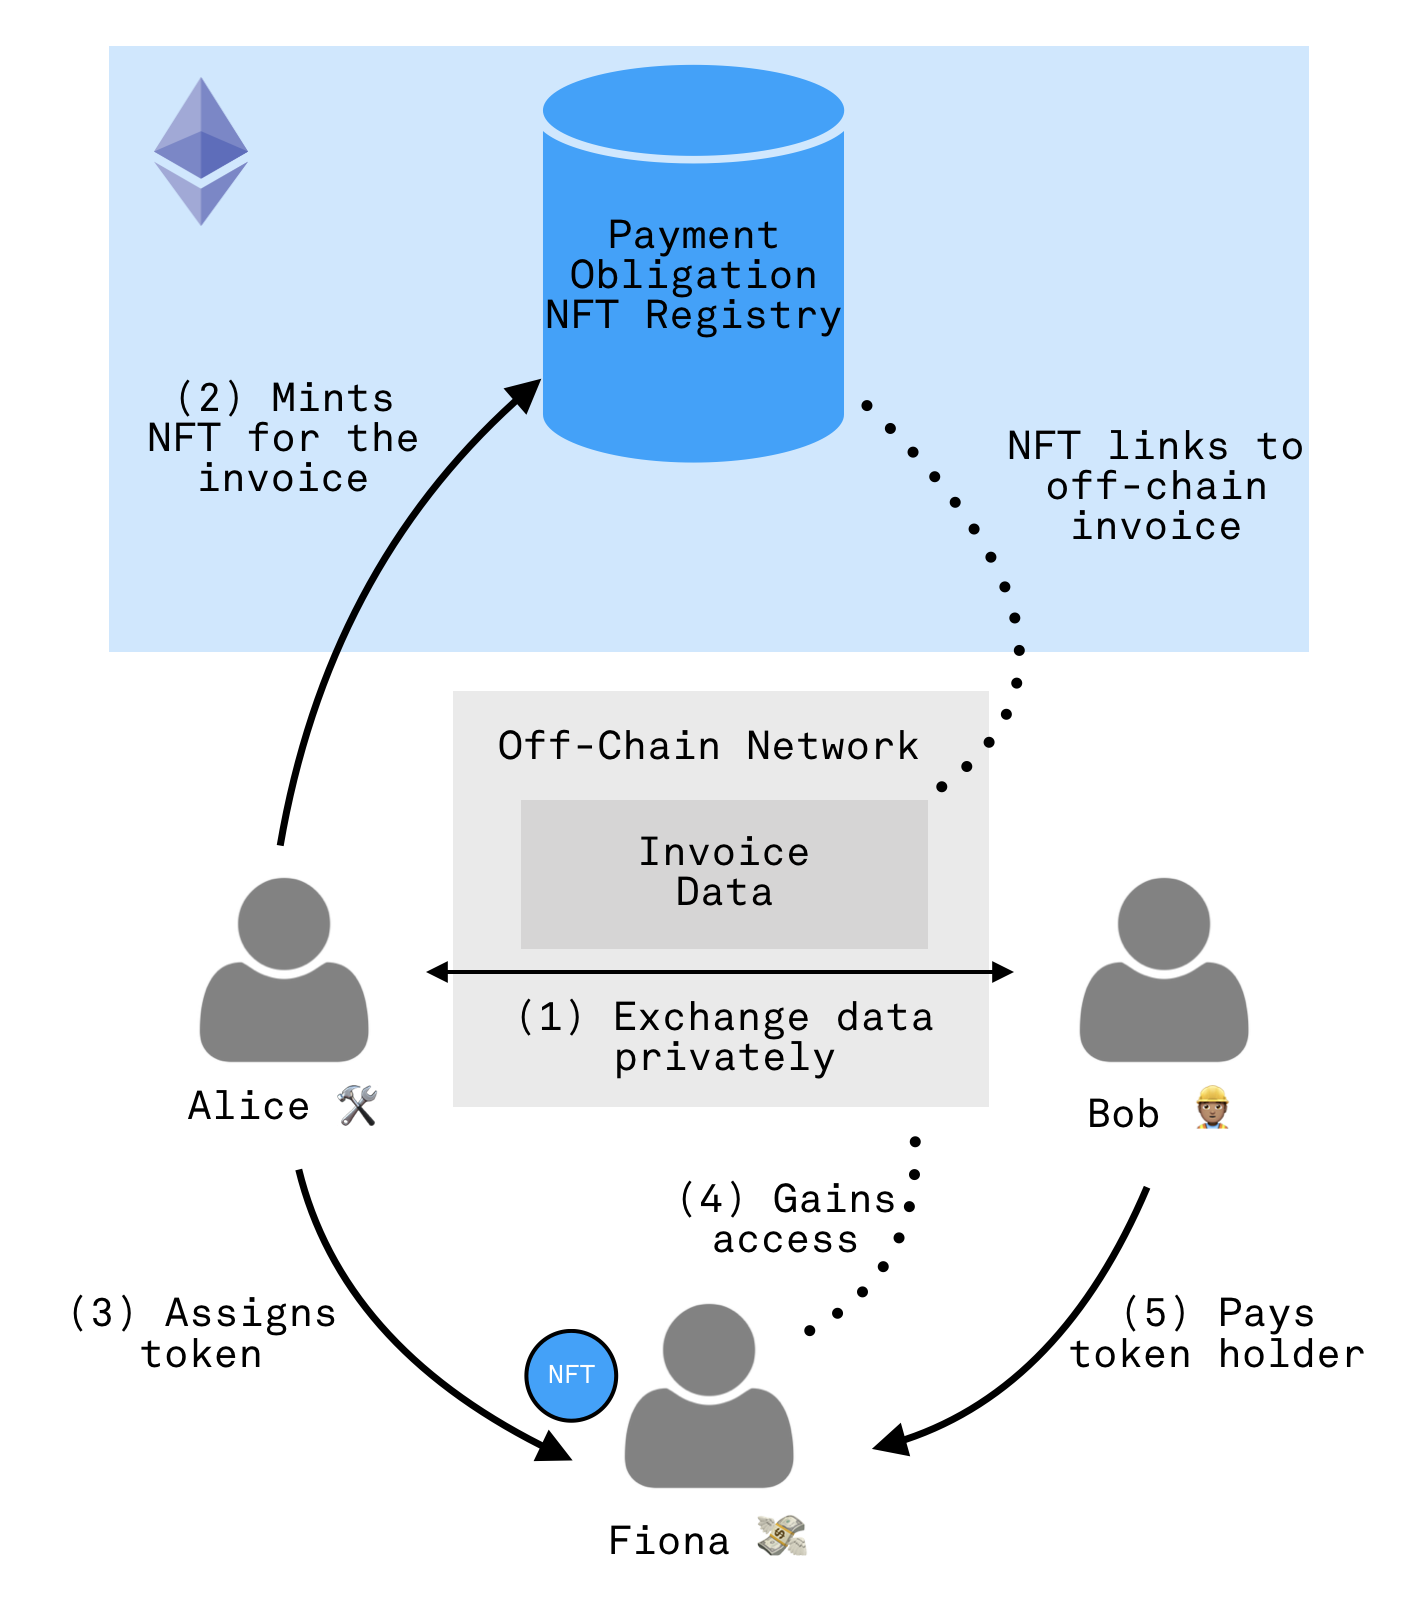
\includegraphics[width=11cm]{drawings/introduction.png}
  \caption{NFTs are minted from off chain data.} 
  \label{introduction}
\end{figure}

Alice mints this token by providing a precise-proof, proving that Bob received the invoice and that she is the supplier of this document. After validating the proofs, the registry assigns the newly minted token to Alice’s wallet address. Once the token is minted and assigned to Alice’s wallet, she can now transfer the NFT to the wallet address of the funder of her choice, Fiona, in return for a financing of the unpaid invoice. As Fiona’s wallet holds the NFT, she will not only receive the payment of the invoice upon due-date but can also create a request for the off-chain data to track any changes to the invoice (e.g., if Bob rejects the invoice, or marks the amounts down) and act accordingly.

\section{Implementation}
The implementation in this paper focuses on the on chain contracts and makes certain assumptions about the off-chain component. Our implementation examples might refer to details of Centrifuge OS. While some details of the implementation are specific to the Centrifuge OS data structures and its peer-to-peer (P2P) network, any off-chain data store can be adapted to the concept of privacy-enabled NFTs.

\subsection{About Centrifuge OS}
Centrifuge OS is a decentralized platform for the financial supply chain. It allows participants to exchange private data (invoices, purchase orders, company master data, etc.) verifiably and securely while supporting on-chain document validation and decentralized access to document data. It implements a combination of Ethereum contracts and a P2P network. The P2P network allows users to privately exchange documents and implements a consensus algorithm that assures agreement on the document state for all involved parties. For every state update, each participant in the transaction signs the Merkle root (created via precise-proofs) of the document, thus indicating consensus on the state of the network. The consensus rules are quite simple and intentionally do not have any outside parties to ensure full privacy between the parties that transact a specific document. To transact on the network a user first registers a simple identity (Centrifuge ID) on Ethereum through a Centrifuge OS contract. The Centrifuge ID is then used by the user to identify themselves on the P2P layer. The on-chain identity allows for attaching public keys corresponding to the private keys that are used on the P2P layer to sign transactions. The public identity, combined with their public keys, is also used to resolve the network addresses of a participant’s node on the P2P layer. If a node requests a document on the P2P layer and the requesting identity is listed in the list of authorized participants of a specific document, the queried node answers such a request. 

\begin{figure}[thpb]
  \centering
  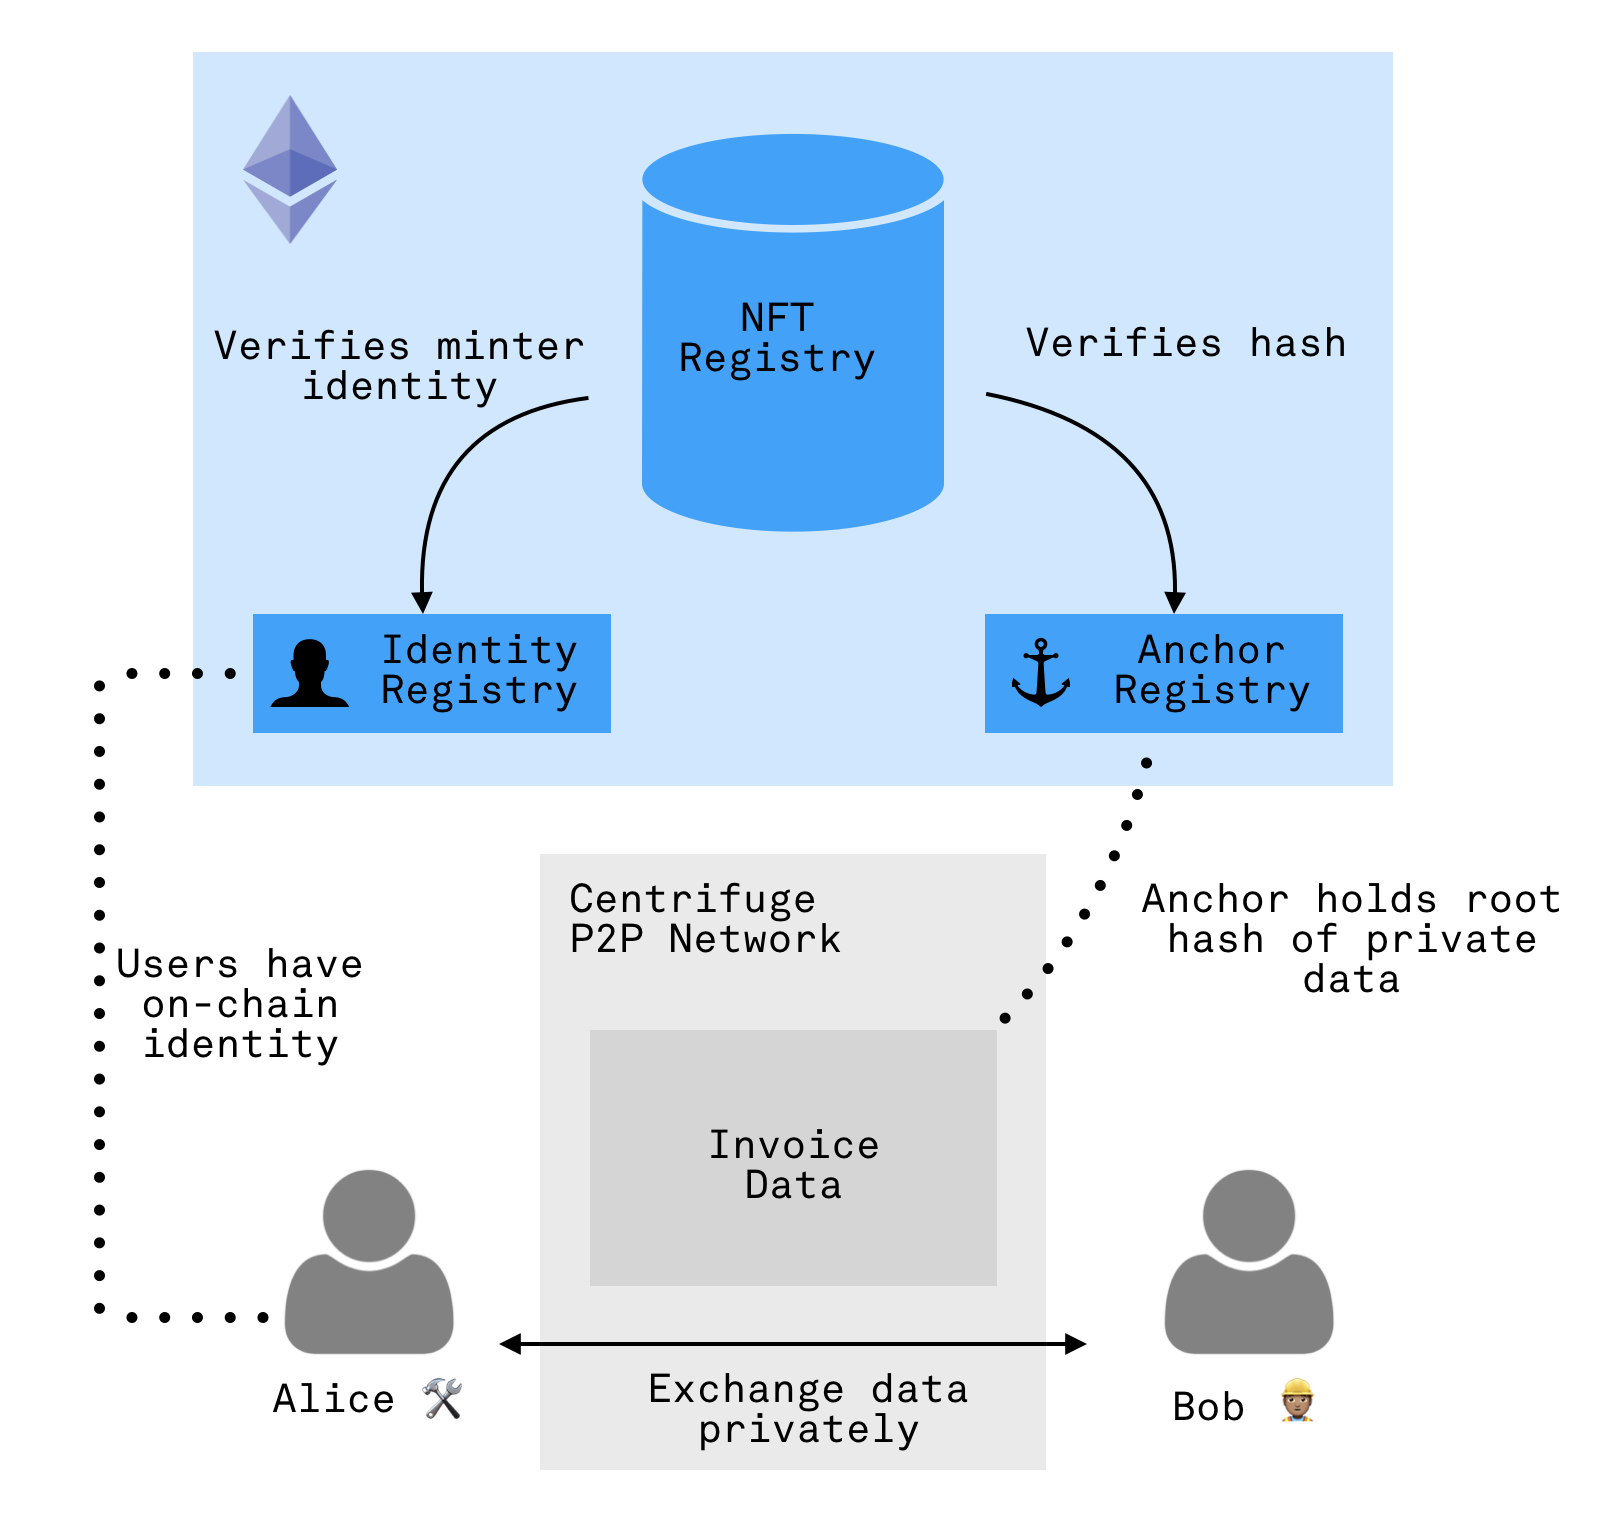
\includegraphics[width=11cm]{drawings/cent_os_overview.png}
  \caption{Simplified Centrifuge OS Architecture.} 
  \label{cent_os_overview}
\end{figure}

\subsection{Verifying Off-Chain Data On Chain With Committed Merkle Roots}
A privacy-enabled NFT registry needs to prove the authenticity of a mint-request reliably. Before minting an NFT for any document, the registry verifies the provided Merkle proof and the root hash of the given document. The registry requires an on-chain “source of truth” against which it compares the provided root hash and the Merkle proof.

Centrifuge OS offers this on-chain verifiability by creating a Merkle tree for each document and committing the document Merkle root on the public chain as part of the P2P document consensus. This enables the creation of Merkle proofs for individual fields that can be verified against the root stored on chain. The precise-proofs library is used to flatten the document structure and calculate the root hash. In Centrifuge OS we call this list of Merkle roots the “anchor registry”. The anchor registry is a mapping of a unique document ID to the document root hash. 

The NFT contracts can, by checking these proofs, verify the authenticity of a mint-request on-chain. When someone tries to mint an NFT for a given document ID, the NFT contract calls the document registry to validate the document hash for the given ID.

\subsection{Required Off-Chain Document Data Schema}
The off-chain document store needs to be able to reliably decide if a request for document data should succeed or fail. To guarantee this consistency, the off-chain data store registers which NFTs currently exist for a given document. In the case of Centrifuge, each document is already represented and exchanged in a structured format between network participants. This format contains document consensus information, collaborator identification, as well as the document data itself. To allow any document collaborator to verify incoming requests from NFT owners, the document data contains a list of the NFT registries and the serial numbers of the NFTs minted for the respective document. In short, an off-chain document holds pointers to the NFTs that represent different parts of the document. 
\subsection{Different Tokens For One Document}
Each token representing a document needs to have a clear indication of its purpose. As an example, there can be multiple NFTs representing a single invoice document. One NFT could represent the future payment obligation while another NFT could be minted once an invoice is paid. This “Paid Invoice NFT” could, for example, be the payment confirmation for a hotel room bill and then be used to unlock a room or consume a service. To allow for this multitude of representations, each NFT registry needs to have clearly defined criteria for the objects it registers as NFTs and the resulting token’s meaning.
 
Different NFTs can also grant different levels of access to the off-chain data. E.g., the holder of a Payment Obligation NFT would have different rights to modify/update/read the off-chain document than the holder of the Paid Invoice NFT that is used to unlock the doors in a hotel. Generally, there should only be one NFT in existence per document (e.g., invoice) and type (e.g., payment obligation) tuple.

\subsection{Document Schema}
In Centrifuge OS, the P2P document metadata contains info about the document's tokenized representations. The section called \texttt{onChainRegistrations} holds the link from document to NFTs.
\sbline
\begin{lstlisting}
{
	"documentIdentifier": "0x...",
    // [...]
 	"onChainRegistrations": [
		// Registration:
		{
			"type": "0x...", // uint256
			"registry": "0x...", // address (20byte)
			"tokenID": "0x..." // uint256
			"concatRegistration": "..." // string
		},
	]
	// [...]
}
\end{lstlisting}

\noindent\begin{tabularx}{\linewidth}{ l X }
\texttt{type} & Identifier of the token definition. Can be namespaced to avoid collisions\\
\texttt{registry} & Ethereum address of the ERC-721 compatible contract\\
\texttt{tokenID} & the token id used to identify this document inside the ERC-721 contract \\
\texttt{concatRegistration} & This field is a performance optimization. To reduce the number of leaves to be proven in the mint-proof this field contains all three fields of the registration concatenated \\
\end{tabularx}

\subsection{Minting Of A Privacy-Enabled NFT}
ERC-721 does not prescribe a specific method to mint NFTs. To mint a new privacy enabled NFT, the contract should expose the following method.

\subsubsection{mint Method}
\codesection{\lstinline[language={}]|function mint(uint256 \_tokenId, address _to, unit256[3] \_registrationLeaf, uint256[] \_registrationProof, [... extra args]) external payable|}

The mint method can specify \texttt{extraArgs} for additional data that can be passed into the method to verify use case specific rules.

The mint method on the NFT registry contact validates the document and ensures a document can only be registered once. If all checks pass, the registry mints the NFT and deposits it into the wallet specified by the caller of the mint method.

\begin{enumerate} 
\item \texttt{\_tokenId} Check: It looks at the mapping of assigned token ids and ensures the \texttt{\_tokenId} is unused. 

\item Verifying the registration: The purpose of this check is to assure that there is no other token of this type minted for this document. The check confirms that the document itself already registers the intent to mint the coin. Specifically, it evaluates the fields defined in the section “Document Schema”. The check is performed by concatenating the three \texttt{\_registrationLeaf} values (type, registry, tokenId) and verifying the Merkle proof (\texttt{\_registrationProof}) for it. 

\item Use-case specific mint rules: Different registries enforce different rules. Those rules depend on the semantic meaning of the NFT. It is up to the implementer to define additional arguments for proofs. 

\end{enumerate}
\subsubsection{Application Specific NFT Minting Rules}
The NFT registry contract contains rules that allow the creation of the NFT from an off-chain document. The “registration” item in the off-chain document has a specific format and is somewhat standardized, but in addition to these checks, the NFT registry can implement others such as:

\begin{itemize}
\item The contract verifies that the owner has a designated role on the off-chain document and is authorized to mint the NFT (e.g., only the supplier can mint the NFT for an Invoice)
\item All involved parties have signed the document state (e.g., buyer \& supplier)
\end{itemize}

\subsection{Granting Document Access To NFT Owners}
A feature of ERC-721 is to create NFTs that are freely assignable and transferable to other Ethereum addresses. These addresses can be different from the initial group of off-chain document collaborators or the off-chain asset creators. Therefore, anyone who can prove ownership of the NFT that represents the off-chain document should receive access to the off-chain data. The ERC-721 standard defines the following interface:

\codesection{\lstinline[language={}]|function ownerOf(uint256 \_tokenId) external view returns (address);|}

The off-chain data store can verify that any incoming request for document details was signed by the private key that corresponds to the \texttt{address} returned by the \texttt{ownerOf} function. 

The general flow of off-chain access verification is as follows:
The NFT owner, Alice, signs a data request with the private key associated with the account that currently owns the NFT
Alice sends this signed off-chain data request to Bob who holds the data
Bob inspects the incoming request and validates that the signature corresponds to the public key of the account that holds the NFT
In case of a valid signature, Bob responds with the document data

We call this type of access control \textit{chain delegated permissioning}.

\subsection{Finding And Accessing The Off-Chain Data}
ERC-721 offers a way for an NFT contract to provide metadata about a token. Explicitly, it defines the function 

\codesection{\lstinline[language={}]|function tokenURI(uint256 \_tokenId) external view returns (string);|}

which points to the location of the token’s metadata. The specification of ERC-721 outlines a response-format to provide such metadata. We extend this response by introducing a new property called \texttt{offChainLocation}. Resulting in this metadata format:\sbline


\begin{lstlisting}[language=JavaScript]
{
    "title": "Asset Metadata",
    "type": "object",
    "properties": {
        "name": {
            "type": "string",
            "description": "Identifies the asset to which this NFT represents",
        },
        "description": {
            "type": "string",
            "description": "Describes the asset to which this NFT represents",
        },
        "image": {
            "type": "string",
            "description": "A URI pointing to a resource with mime type image/* representing the asset to which this NFT represents. Consider making any images at a width between 320 and 1080 pixels and aspect ratio between 1.91:1 and 4:5 inclusive.",
        },
        "offChainLocation": {
            "type": "string",
            "description": "A RFC 3986 compliant URI pointing to the off-chain location for the given token.",
        }
    }
};
\end{lstlisting}

In the case of Centrifuge OS, the \texttt{offChainLocation} URI of an asset is a combination of the document identifier and the Centrifuge ID of a P2P network participant who holds the private data. 
For example:

\codesection{\lstinline[language={}]|centrifuge://<P2P Network Participant ID>/<document identifier>|}

For the NFT owner, Fiona, to request the document data she follows these steps:
\begin{enumerate}
    \item Fiona, reads function \texttt{tokenURI(uint256 \_tokenId)} external view returns a string with the token URI of her token.
    \item She calls the returned URI to retrieve the NFT meta-data and inspects the property \texttt{offChainLocation} in the returned JSON and uses this URI to create the following request
    \item Fiona signs her data request with the private key associated with the account that currently owns the NFT. This account is also registered on Fiona’s Centrifuge ID as a valid account for P2P communication.
    \item Fiona sends this signed off-chain data request via the Centrifuge P2P layer to the URI as defined in the asset’s metadata. In this case, the request goes to Bob who holds the data. Requests on Centrifuge always include a signature of the caller. With that, the request uniquely identifies the caller being Fiona, as identified by her signature as part of the request
    \item Bob inspects the incoming request and determines that the request came from a key that is associated with a Centrifuge ID that was initially not part of the document collaborators but instead coming from a Centrifuge ID, claiming to have access to the document data, as dictated by the NFT ownership.
    \item Bob validates that the request’s signature was generated with a private key that corresponds to an authorized public key as listed on the caller’s Centrifuge ID. Centrifuge OS specifications dictate that only requests from valid Centrifuge IDs are answered.
    \item Bob validates that the key that was used to sign the message corresponds to the current owner/approved operator of the NFT by calling
        \begin{enumerate}
            \item \texttt{function ownerOf(uint256 \_tokenId) external view returns (address);}
            \item \texttt{function getApproved(uint256 \_tokenId) external view returns (address);}
            \item \texttt{function isApprovedForAll(address \_owner, address \_operator) external view returns (bool);}
        \end{enumerate}
    In the case of a valid signature, valid association of the account to Centrifuge ID, and valid ownership/approval on the NFT, Bob responds with the document data.

\end{enumerate}

\section{Use-case: Converting an invoice into an NFT to access financing}
Below is a walk through the detailed steps of the whole process, let’s look at the invoice financing example again.

\begin{figure}[thpb]
  \centering
  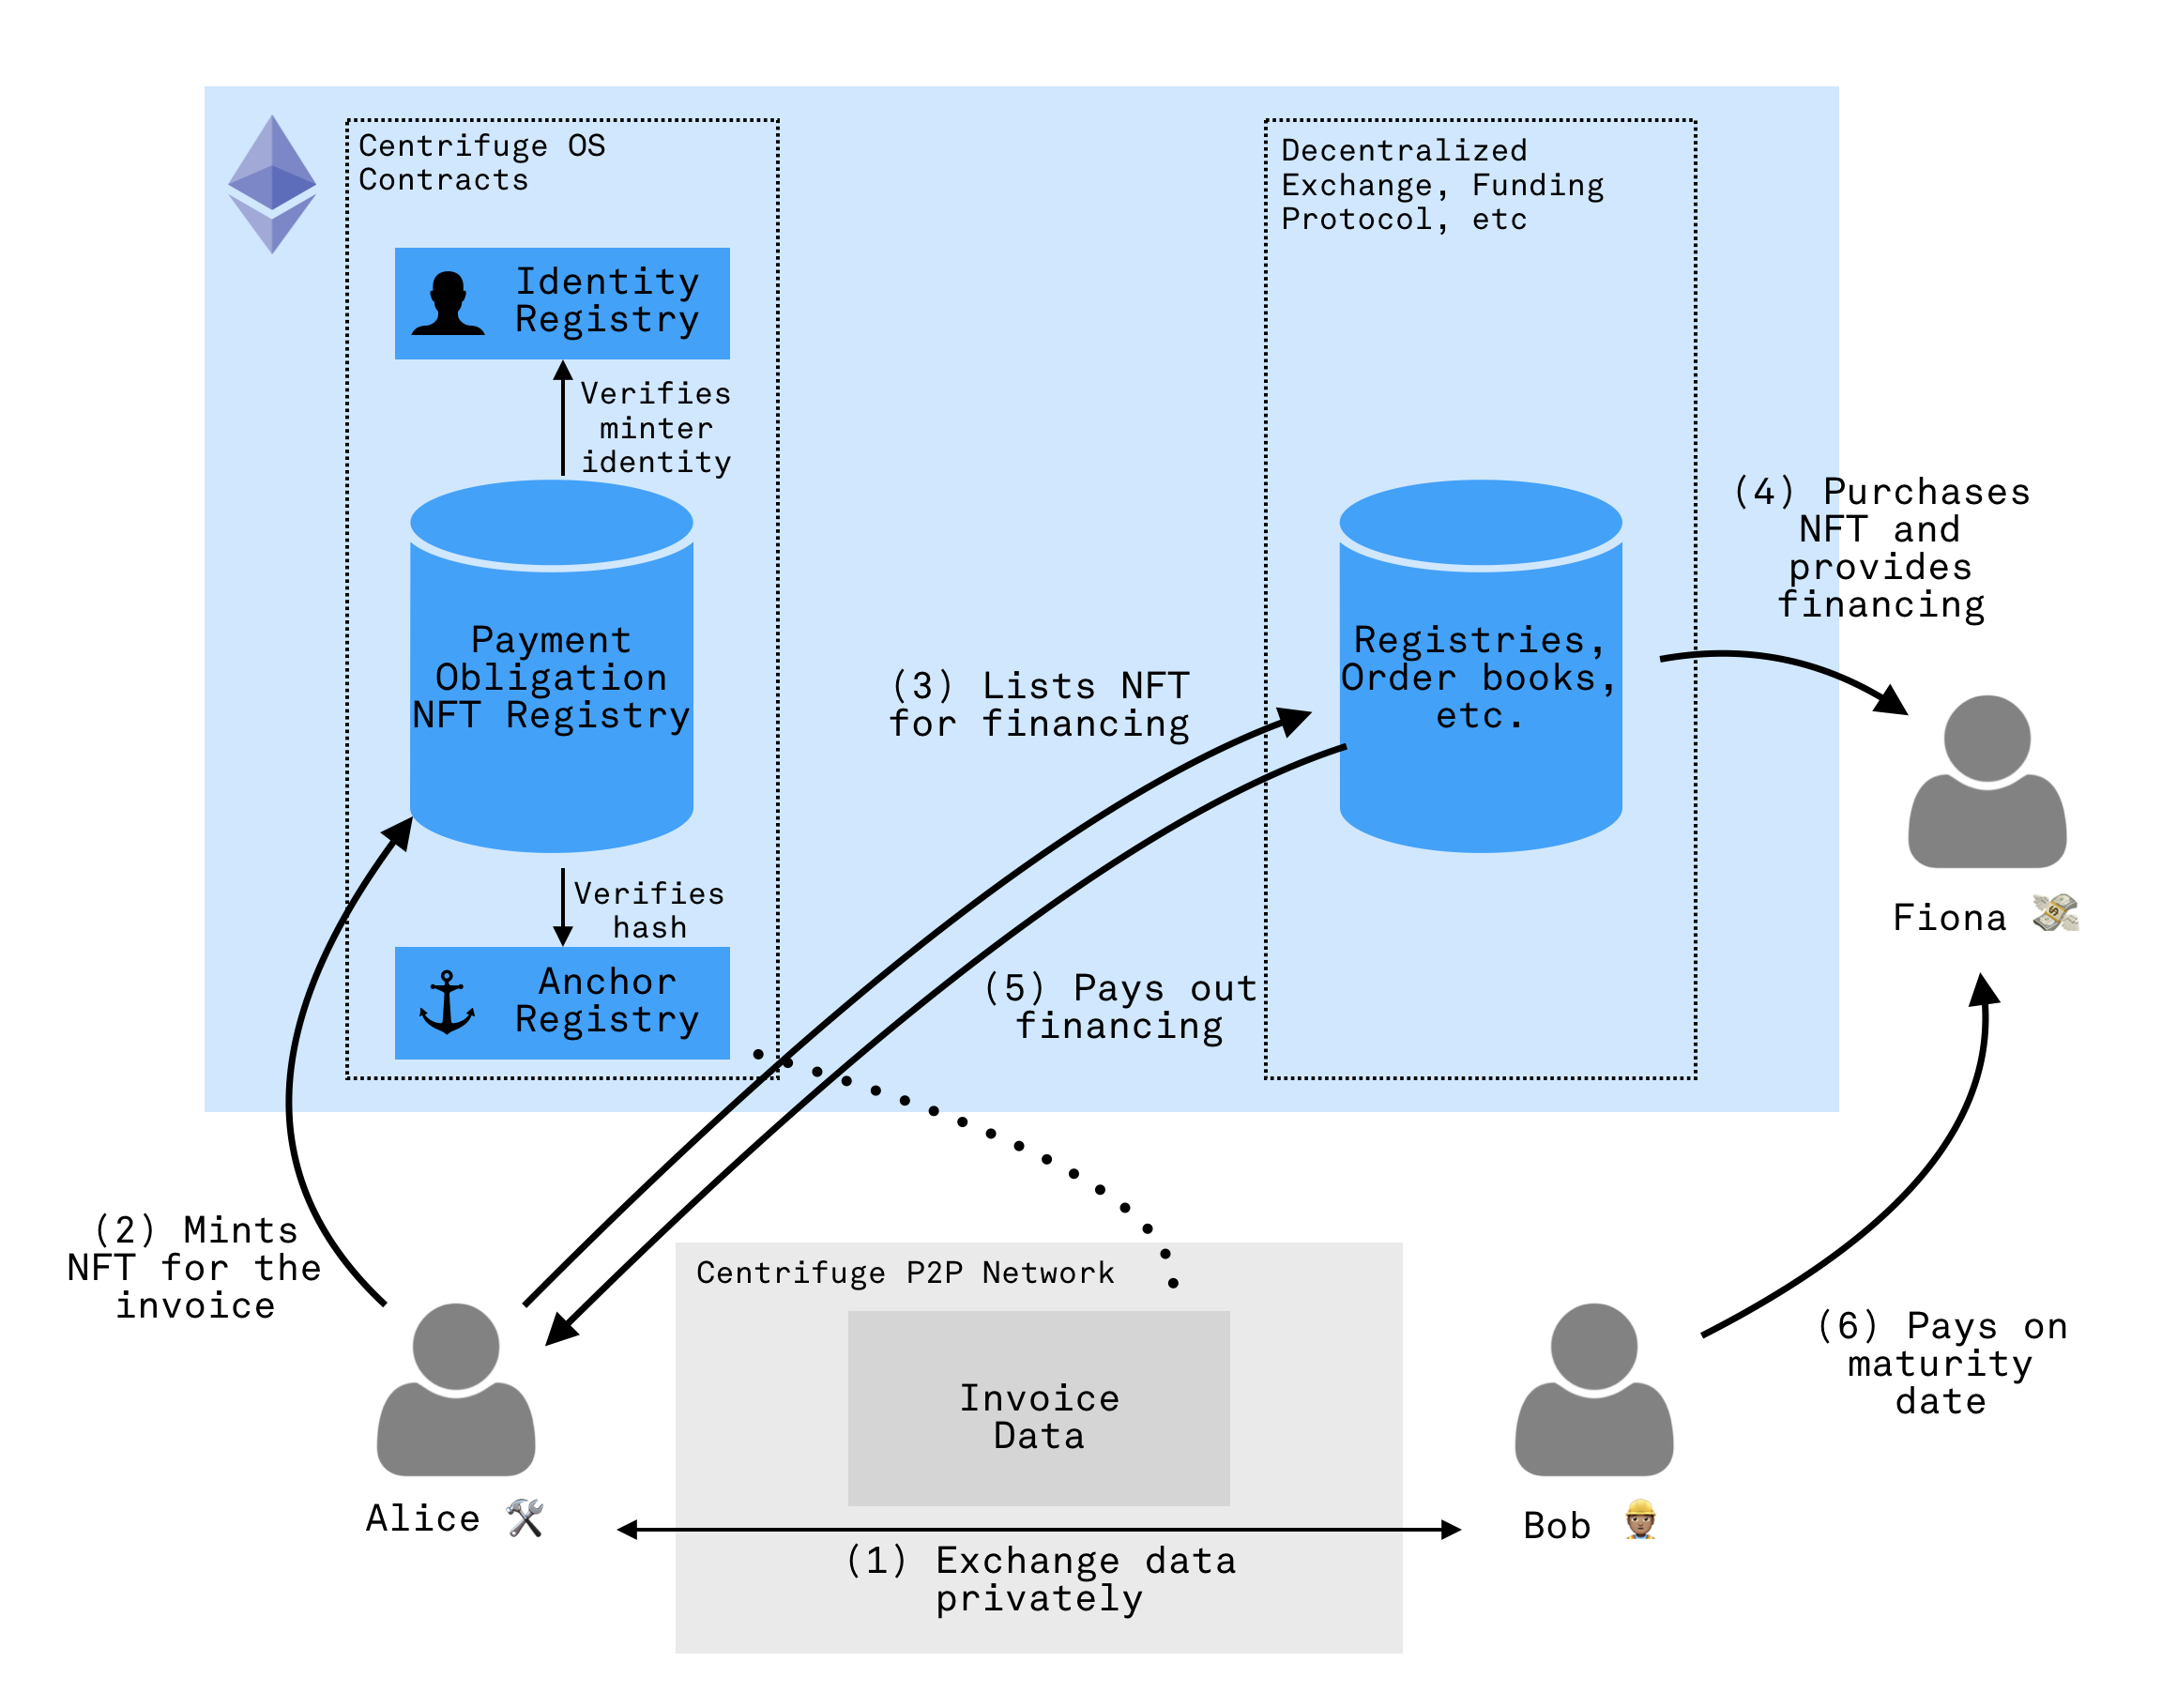
\includegraphics[width=15cm]{drawings/funding_marketplace.png}
  \caption{Invoice Financing NFTs} 
  \label{funding_marketplace}
\end{figure}

\begin{enumerate}
    \item A supplier, Alice, and her customer, Bob exchange an invoice on the Centrifuge OS P2P layer. 
    \begin{enumerate}
        \item During this exchange, Alice and Bob sign the document content via precise-proofs with their keys, associated with their on-chain Centrifuge OS identities. A document anchor is created on Ethereum to identify this signed document state. 
        \item Bob accepts the invoice with an agreed due date and sends this signed data via the P2P layer to Alice. A new version of the document state is anchored on-chain.
    \end{enumerate}
    
    \item Alice registers an NFT representing the payment obligation for this invoice by calling the payment obligation NFT registry’s mint method. In this case, the contract is a Centrifuge OS contract. The token uniquely identifies the fact that when Bob pays this invoice at some point in the future, the then holder of the NFT will receive the payment. To mint the token Alice follows these steps:
    \begin{enumerate}
        \item Alice creates and signs an update to the invoice document on the P2P layer assigning the ownership of the payment obligation to the NFT contract address. The document update assures that the P2P layer is aware of an NFT about to be registered. It also guarantees the creation of a record for the future payment routing (upon invoice due-date).
        \item Alice creates an Ethereum transaction containing precise-proofs for this document and sends the transaction to the NFT contract. This transaction will mint the token. The transaction contains the following information/proofs:
        \begin{enumerate}
            \item The document identifier as identified on the P2P layer and registered on the on-chain anchor registry
            \item Prove that: The document contains Alice’s Centrifuge ID as the “supplier”. The supplier is the original recipient of the payment if there would be no NFT involved. This registry will only issue the token to the original supplier.
            \item Prove that: The payment obligation is assigned to the NFT contract’s address.
            \item other rules/data as needed
        \end{enumerate}
        \item The contract verifies the precise proof and mints the Payment Obligation NFT, assigning it to Alice’s wallet address. The contract performs validations like:
        \begin{enumerate} 
            \item Check that sender of the Ethereum transaction is an address associated to the supplier’s Centrifuge ID
            \item Check that the proof’s root matches the root hash of the document ID as listed on the anchor registry
            \item other validations as needed
        \end{enumerate}
    \end{enumerate}
    \item Alice can now trade this Payment Obligation NFT at a (decentralized) exchange, funding marketplace, lending marketplace, or other systems that support ERC-721s to gain access to liquidity for this unpaid invoice.\sbline
Note that Privacy-Enabled NFTs do not prescribe the discovery and trading mechanisms. However, a buyer of an NFT might require specific additional metadata about an asset that they want to acquire before they would purchase it. There are various mechanisms to achieve this, but that is outside of the scope of this paper.
    \item A funder, Fiona, purchases the Payment Obligation NFT and with that provides financing that can be distributed to Alice
    \item Alice receives the requested financing
    \item Once the invoice becomes due, the buyer, Bob, will pay whoever owns the Payment Obligation NFT then
\end{enumerate}

\section{Limitations And Attack Vectors}
\subsection{Different Use-Cases == Different Registries And Requirements}
The approach of minting privacy-enabled NFTs does not dictate specific business logic that goes into the minting of the token itself. The approach also does not prescribe what is or what isn’t possible with the minted NFT. The schema for validating off-chain data through precise-proofs and granting off-chain document access based on NFT ownership applies to many use-cases and a general tool. The actual implementation is required to follow their application, business, and legal requirements.
E.g., to finance a Payment Obligation NFT (the example in this document) the funder still needs to assure that their legal requirements are met (on-chain and off-chain) to make such a funding legally binding within their jurisdiction. 
\subsection{Withholding Off-Chain Data Requests}
Depending on the implementation of the off-chain datastore a data-owner might have the ability to withhold data that is being requested by the current owner of an NFT. The actual data store could be centrally managed and operated (e.g., a central “document API” that provides data access to the NFT holder) or it could be a decentralized network where the data holders are incentivized or financially rewarded to provide data to the NFT holder. In any case, the suggested approach to privacy-enabled NFTs does not dictate the actual implementation of the off-chain data store and with that cannot guarantee the data availability to the token holder itself.
Examples of decentralized, incentivized off-chain data stores are IPFS or FileCoin. Those would still require a layer of encryption and access-control to assure only authorized holders of an NFT can access the off-chain data or mint the NFT in the first place.
An encrypted, decentralized off-chain data store such as NuCypher could provide encrypted, private off-chain data but still requires a layer to interface with the NFT contracts as well as a layer that coordinates and validates data access requests coming from NFT holders.

% TODO
\printacronyms[include-classes=abbrev,name=Abbreviations]

\printacronyms[include-classes=nomencl,name=Nomenclature]


\end{document}

